%%%%%%%%%%%%%%%%%%%%%%%%%%%%%%%%%%%%%%%%%
% Beamer Presentation
% LaTeX Template
% Version 1.0 (10/11/12)
%
% This template has been downloaded from:
% http://www.LaTeXTemplates.com
%
% License:
% CC BY-NC-SA 3.0 (http://creativecommons.org/licenses/by-nc-sa/3.0/)
%
%%%%%%%%%%%%%%%%%%%%%%%%%%%%%%%%%%%%%%%%%

%----------------------------------------------------------------------------------------
%	PACKAGES AND THEMES
%----------------------------------------------------------------------------------------

\documentclass{beamer}

\mode<presentation> {
	\usepackage[utf8]{vietnam}
	\newcommand\tab[1][1cm]{\hspace*{#1}}
	\graphicspath{ {images/} }
	% The Beamer class comes with a number of default slide themes
	% which change the colors and layouts of slides. Below this is a list
	% of all the themes, uncomment each in turn to see what they look like.
	
	%\usetheme{default}
	%\usetheme{AnnArbor}
	%\usetheme{Antibes}
	%\usetheme{Bergen}
	%\usetheme{Berkeley}
	%\usetheme{Berlin}
	%\usetheme{Boadilla}
	%\usetheme{CambridgeUS}
	%\usetheme{Copenhagen}
	%\usetheme{Darmstadt}
	%\usetheme{Dresden}
	%\usetheme{Frankfurt}
	%\usetheme{Goettingen}
	%\usetheme{Hannover}
	%\usetheme{Ilmenau}
	%\usetheme{JuanLesPins}
	%\usetheme{Luebeck}
	\usetheme[secheader]{Madrid}
	%\usetheme{Malmoe}
	%\usetheme{Marburg}
	%\usetheme{Montpellier}
	%\usetheme{PaloAlto}
	%\usetheme{Pittsburgh}
	%\usetheme{Rochester}
	%\usetheme{Singapore}
	%\usetheme{Szeged}
	%\usetheme{Warsaw}
	
	% As well as themes, the Beamer class has a number of color themes
	% for any slide theme. Uncomment each of these in turn to see how it
	% changes the colors of your current slide theme.
	
	%\usecolortheme{albatross}
	%\usecolortheme{beaver}
	%\usecolortheme{beetle}
	%\usecolortheme{crane}
	%\usecolortheme{dolphin}
	%\usecolortheme{dove}
	%\usecolortheme{fly}
	%\usecolortheme{lily}
	%\usecolortheme{orchid}
	%\usecolortheme{rose}
	%\usecolortheme{seagull}
	%\usecolortheme{seahorse}
	%\usecolortheme{whale}
	%\usecolortheme{wolverine}
	
	%\setbeamertemplate{footline} % To remove the footer line in all slides uncomment this line
	%\setbeamertemplate{footline}[page number] % To replace the footer line in all slides with a simple slide count uncomment this line
	
	%\setbeamertemplate{navigation symbols}{} % To remove the navigation symbols from the bottom of all slides uncomment this line
}

\usepackage{graphicx} % Allows including images
\usepackage{booktabs} % Allows the use of \toprule, \midrule and \bottomrule in tables
\usepackage{caption}
\usepackage{fancyvrb}
\usepackage{bbm}
\everymath{\color{blue}}%make in-line maths symbols blue to read/check easily

%\sloppy
\captionsetup[figure]{labelfont={small,bf},textfont={small,it},belowskip=-1pt,aboveskip=-9pt}

\captionsetup[table]{labelfont={small,bf},textfont={small,it},belowskip=-1pt,aboveskip=7pt}
%----------------------------------------------------------------------------------------
%	TITLE PAGE
%----------------------------------------------------------------------------------------

\title[Nhận dạng biểu thức toán học]{ Nhận dạng biểu thức toán học}


\author[Phan Tấn Phúc - Bùi Khánh Ngọc]{} % Your name
\institute[BKU] % Your institution as it will appear on the bottom of every slide, may be shorthand to save space
{
	\bf{Đại học Bách Khoa Thành phố Hồ Chí Minh} \\ % Your institution for the title page
	\medskip
	\bf{Khoa Khoa Học và Kỹ Thuật Máy Tính}\\
	\medskip
	\textit{\{phantanphuc2512, buikhanhngoc142\}@gmail.com} % Your email address
}

\date[\today]{} % Date, can be changed to a custom date
\logo{
\includegraphics[height=1cm]{hcmut.png}}
\begin{document}
\begin{frame}[plain]
\maketitle
\small
{\centering\itshape \huge{\bf{Luận văn tốt nghiệp đại học}} \par}
\footnotesize
\begin{table}[c]
	\begin{tabular}{rrl}
		%\vspace{0.5cm}
		\hspace{1.5 cm} & Hội đồng & : \bf{Khoa học máy tính}\\
		%	\vspace{0.5cm}
		\hspace{1.5 cm} & Giảng viên hướng dẫn & : \bf{TS. LÊ Thành Sách}\\
		%\vspace{0.5cm}
		\hspace{1.5cm} & Giảng viên phản biện & : \bf{TS. Nguyễn Đức Dũng}\\
		%\vspace{0.5cm}
		\hspace{1.5 cm} & Nhóm sinh viên thực hiện & : \bf{Phan Tấn Phúc - 51303058}\\
		%	\vspace{0.5cm}
		\hspace{1.5 cm} & \hspace{5 cm} &  \hspace{0.15cm} \bf{Bùi Khánh Ngọc - 51302567}\\
		
	\end{tabular}
\end{table}
\begin{center}
	{\footnotesize Tp. Hồ Chí Minh, Tháng 01/2018}
\end{center}
\end{frame}

\begin{frame}
\frametitle{Overview} % Table of contents slide, comment this block out to remove it
\tableofcontents[pausesections] % Throughout your presentation, if you choose to use \section{} and \subsection{} commands, these will automatically be printed on this slide as an overview of your presentation
\end{frame}

%----------------------------------------------------------------------------------------
%	PRESENTATION SLIDES
%----------------------------------------------------------------------------------------



\section{Giới thiệu}
%------------------------------------------------

\begin{frame}
\frametitle{Giới thiệu đề tài}
{\Huge Giới thiệu đề tài}
\end{frame}

%---------------------------------------------------

\section{Công trình liên quan}
\begin{frame}
\frametitle{Công trình liên quan}
{\Huge Giới thiệu đề tài}

\end{frame}

%--------------------------------------------------
%--------------------------------------------------
%--------------------------------------------------
%--------------------------------------------------


\section{Mô hình đề xuất}
\begin{frame}
\frametitle{Mô hình đề xuất}
{\Huge Mô hình đề xuất}
\hspace{10 cm}




Mạng SSD - Single Shot Multibox Detector
\end{frame}

%--------------------------------------------------
%----------SUBSEC: SSD----------------------
%--------------------------------------------------
\subsection{Lý thuyết mạng SSD}

\frame{\tableofcontents[currentsection]}

\begin{frame}
\frametitle{Lý thuyết mạng SSD}

SSD\cite{liu2016ssd} sinh ra một số lượng hữu hạn các \textbf{default box}\footnote{Tiếng việt: Ô chuẩn} được xem là các "hệ quy chiếu" để hệ thống có thể xác định vị trí và kích thước các ký tự cần nhận diện. Thông qua quá trình huấn luyện, mạng cần phải học cách dự đoán các \textbf{bounding box}\footnote{Tiếng việt: Ô Bọc} bọc quanh ký tự cần nhận diện thông qua "hệ quy chiếu" tương ứng bên trên.

SSD\cite{liu2016ssd} sử dụng các lớp tích chập\footnote{Thuật ngữ tiếng Anh: Convolution layer} (hay cụ thể hơn là mạng nơ-ron tích chập\footnote{Thuật ngữ tiếng anh: Convolutional neural network}) để trích đặc trưng, tạo tiền đề cho việc phát hiện và phân loại ký tự. \\
%Nhóm xin phép được tách quá trình huấn luyện thành ba giai đoạn: mã hóa, phát hiện - phân loại và tính giá trị lỗi. Và song song với huấn luyện, quá trình kiểm tra, kiểm định, chạy thực tiễn cũng được chia thành ba giai đoạn: trích đặc trưng - phân loại và giải mã. << Talk

\end{frame}

%--------------------------------------------------
%----------SUBSUB: ENCODER----------------------
%--------------------------------------------------

%---------------ENCODER------------------------------

\subsubsection{Bộ Mã Hóa (Encoder)}
\begin{frame}
\frametitle{Bộ Mã Hóa (Encoder) - Sinh Default Box}

\end{frame}

%----------------MATCHING---------------------------

\begin{frame}
\frametitle{Bộ Mã Hóa (Encoder) - Matching}


\begin{center}
\centering
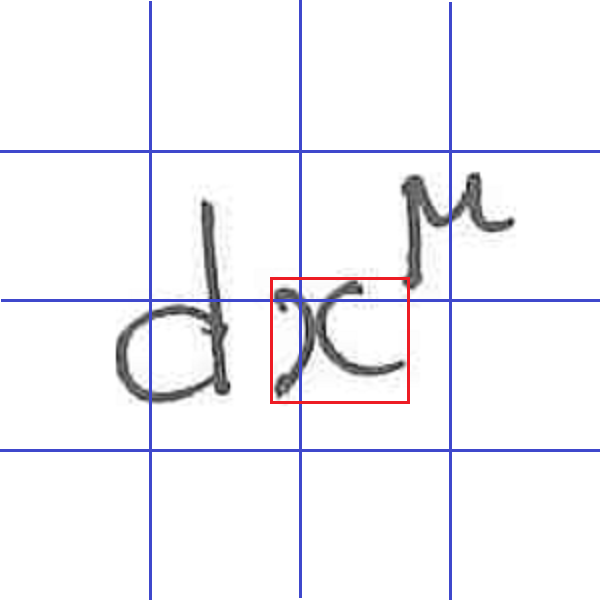
\includegraphics[width=0.6\linewidth]{GT.png}
\captionof{figure}{GT\cite{Jaccard}}
\end{center}

\end{frame}

%--------------------------------------------------
%--------------------------------------------------
%--------------------------------------------------
%--------------------------------------------------

\section{Đánh giá kết quả}
\begin{frame}
\frametitle{Đánh giá kết quả}
{\Huge Đánh giá kết quả}
\end{frame}

\section{Tổng kết}
\begin{frame}
\frametitle{Tổng kết}
{\Huge Tổng kết}
\end{frame}

\begin{frame}
\frametitle{References}
\newpage
\bibliographystyle{ieeetr}
\bibliography{ref}
\end{frame}


%------------------------------------------------

\begin{frame}
\Huge{\centering{The End}}
\end{frame}

%----------------------------------------------------------------------------------------

\end{document}